\documentclass[12pt, a4paper, oneside]{ctexart}
\usepackage{amsmath, amsthm, amssymb, bm, color, graphicx, geometry, mathrsfs,extarrows, braket, booktabs, array, subfigure}
\usepackage[colorlinks,linkcolor=red,anchorcolor=blue,citecolor=blue,urlcolor=blue,menucolor=black]{hyperref}
\setmainfont{Times New Roman}  % 设置英文字体
\setsansfont{Calibri}
\setmonofont{Consolas}

\linespread{1.4}
%\geometry{left=2.54cm,right=2.54cm,top=3.18cm,bottom=3.18cm}
\geometry{left=1.84cm,right=1.84cm,top=2.18cm,bottom=2.18cm}
\newenvironment{problem}{\par\noindent\textbf{题目. }}{\bigskip\par}
\newenvironment{solution}{\par\noindent\textbf{解答. }}{\bigskip\par}
\newenvironment{note}{\par\noindent\textbf{注记. }}{\bigskip\par}

\everymath{\displaystyle} % 默认全部行间公式
\DeclareMathOperator*\uplim{\overline{lim}} % 定义上极限 \uplim_{}
\DeclareMathOperator*\lowlim{\underline{lim}} % 定义下极限 \lowlim_{}
\let\leq=\leqslant % 将全部leq变为leqslant
\let\geq=\geqslant % geq同理
\graphicspath{{figure/}}

% 一些宏定义
\def\bd{\boldsymbol}    % 加粗(向量) boldsymbol
\def\disp{\displaystyle}% 使用行间公式 displaystyle(默认)
\def\tsty{\textstyle}   % 使用行内公式 textstyle
\def\sign{\text{sign}}  % sign function
\def\wtd{\widetilde}    % 宽波浪线 widetilde
\def\R{\mathbb{R}}      % Real number
\def\C{\mathbb{C}}      % Complex number
\def\d{\mathrm{d}}      % differential operator
\def\e{\mathrm{e}}      % Euler's number
\def\i{\mathrm{i}}      % imaginary number
\def\re{\mathrm{Re\,}}    % Real part
\def\im{\mathrm{Im\,}}    % Imaginary part
\def\L{\mathcal{L}}     % Loss function
\def\wdh{\widehat}      % 宽帽子 widehat
\def\ol{\overline}      % 上横线 overline
\def\ul{\underline}     % 下横线 underline
\def\add{\vspace{1ex}}  % 增加行间距
\def\del{\vspace{-3.5ex}}  % 减少行间距

% 基本信息
\newcommand{\RQ}{\today} % 日期
\newcommand{\km}{经济博弈论} % 科目
\newcommand{\bj}{强基数学002} % 班级
\newcommand{\xm}{吴天阳} % 姓名
\newcommand{\xh}{2204210460} % 学号

\begin{document}

%\pagestyle{empty}
\pagestyle{plain}
\vspace*{-15ex}
\centerline{\begin{tabular}{*5{c}}
    \parbox[t]{0.25\linewidth}{\begin{center}\textbf{日期}\\ \large \textcolor{blue}{\RQ}\end{center}} 
    & \parbox[t]{0.2\linewidth}{\begin{center}\textbf{科目}\\ \large \textcolor{blue}{\km}\end{center}}
    & \parbox[t]{0.2\linewidth}{\begin{center}\textbf{班级}\\ \large \textcolor{blue}{\bj}\end{center}}
    & \parbox[t]{0.1\linewidth}{\begin{center}\textbf{姓名}\\ \large \textcolor{blue}{\xm}\end{center}}
    & \parbox[t]{0.15\linewidth}{\begin{center}\textbf{学号}\\ \large \textcolor{blue}{\xh}\end{center}} \\ \hline
\end{tabular}}
\vspace*{4ex}

% 正文部分
\paragraph{第三章}\del
\paragraph{4.}如果开金矿博弈中第三阶段乙选择打官司后的结果尚不能肯定, 即下图\ref{sub@fig-4.1}中$a,b$的数值不确定. 试讨论本博弈中有哪几种可能的结果. 如果要本博弈中的“威胁”和“承诺”是可信的, $a$或$b$应满足什么条件?
\begin{figure}[htbp]
    \centering
    \subfigure[] {
        \label{fig-4.1}
        \begin{minipage}[b]{.45\linewidth}
            \centering
            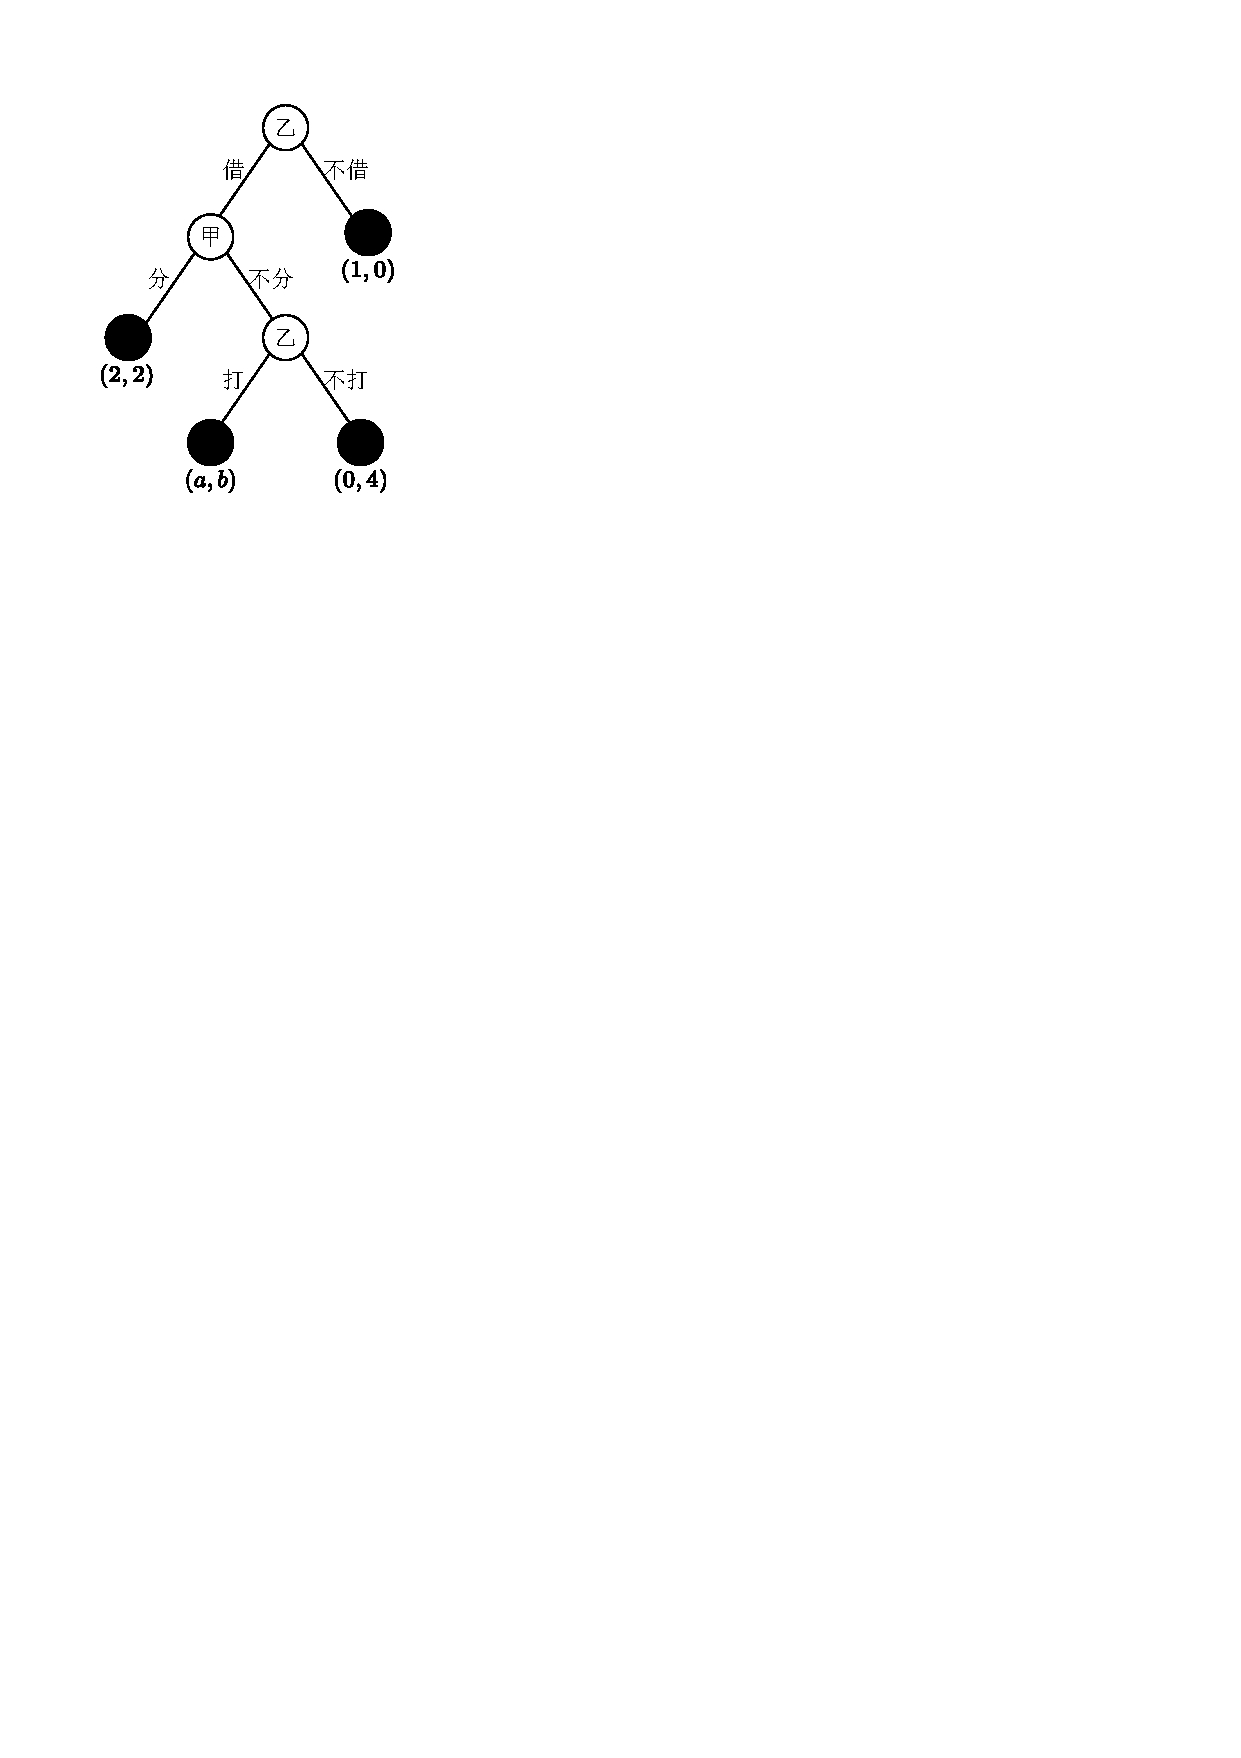
\includegraphics[scale=0.9]{经济博弈论3.4_1.pdf}
        \end{minipage}
    }
    \subfigure[] {
        \label{fig-4.2}
        \begin{minipage}[b]{.45\linewidth}
            \centering
            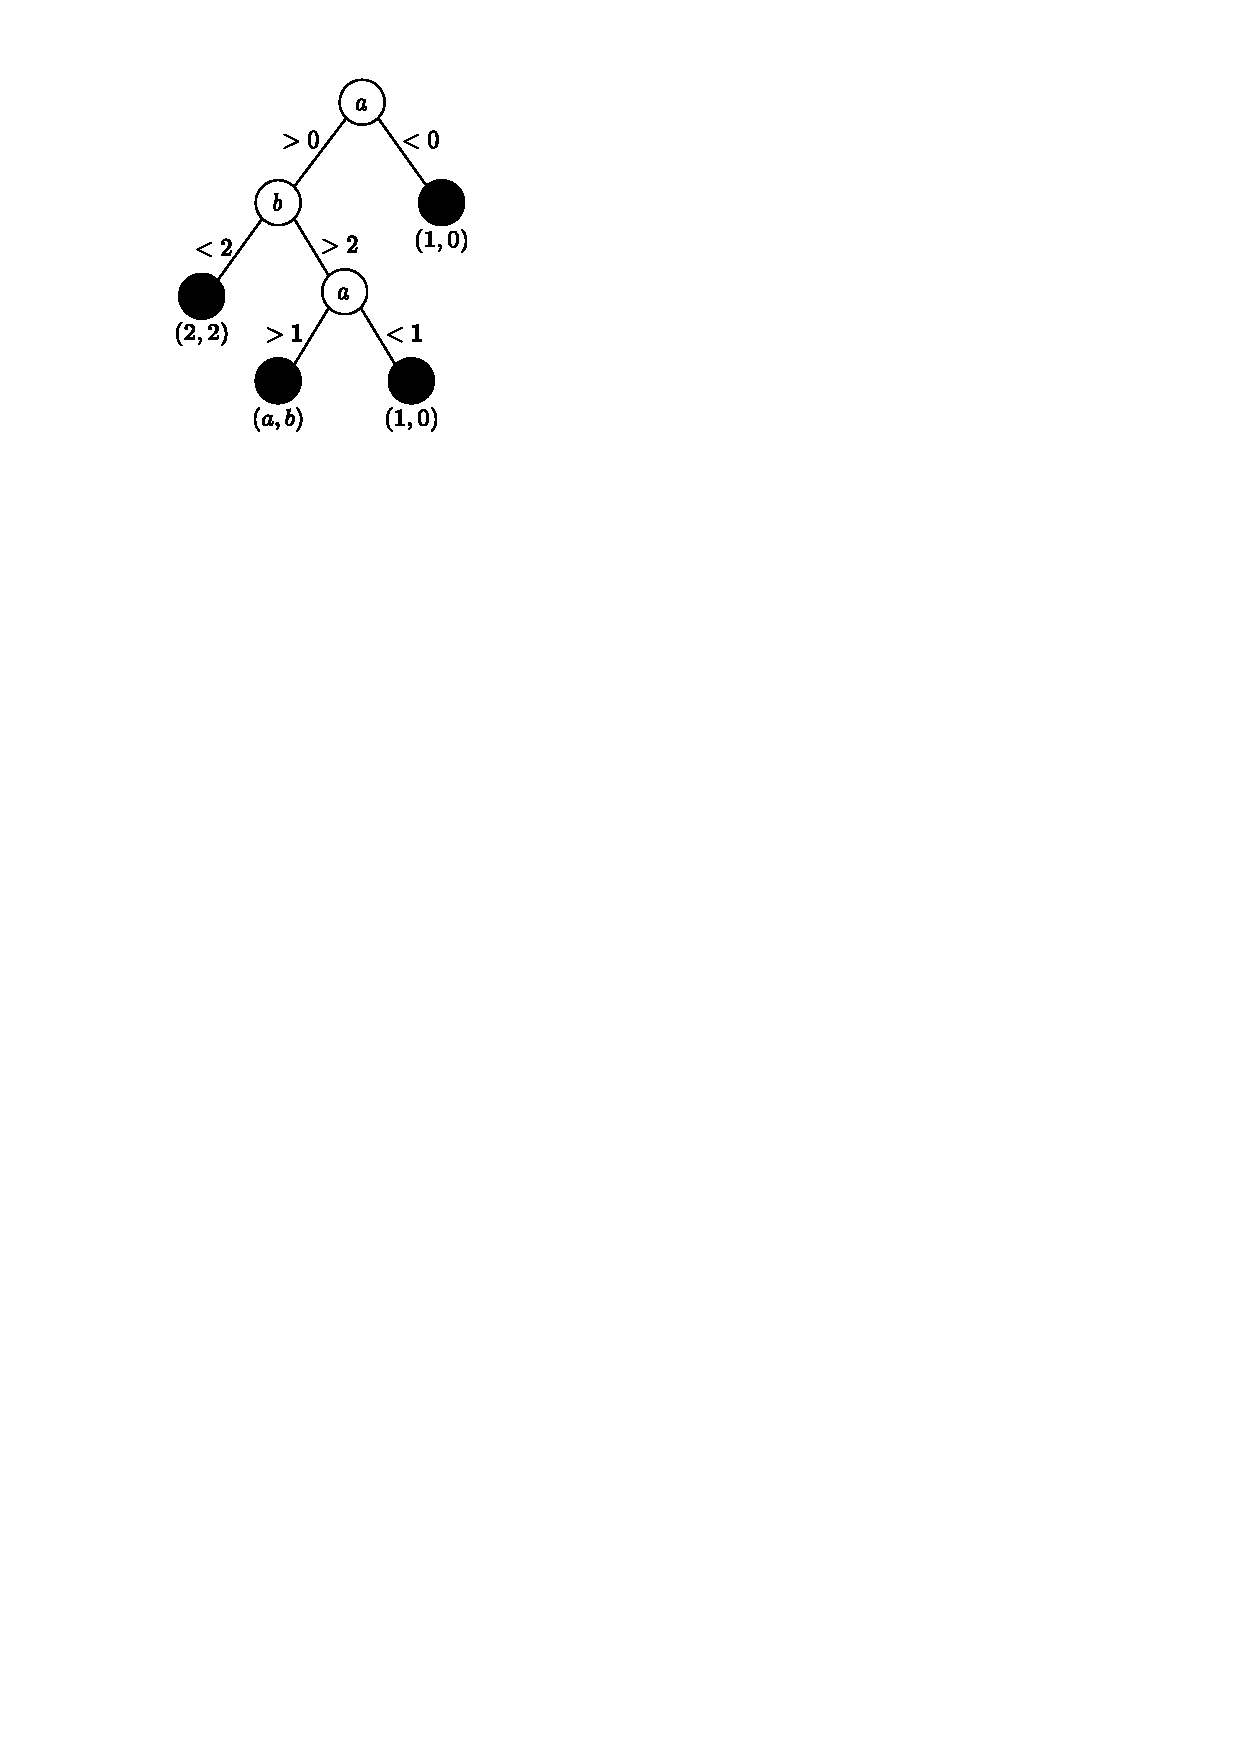
\includegraphics[scale=1]{经济博弈论3.4_2.pdf}
        \end{minipage}
    }
\end{figure}\del
\begin{solution}
    若$a<0$, 则第三阶段乙选择不打官司, 第二阶段甲选择不分金矿, 第一阶段乙选择不借, 不进行合作, 最终双方得益为$(1,0)$. 若$a > 0$, 则第三阶段乙选择打官司, 若$b > 2$, 则第二阶段甲不分金矿, 若$a < 1$, 则第一阶段乙选择不借, 最终双方得益为$(1,0)$; 若$a > 1$, 则第一阶段乙选择借, 最终双方得益为$(a, b)$; 若$b < 2$, 则第二阶段甲分金矿, 最终双方得益为$(2, 2)$. 综上, 可将上述推导绘制成与变量$a, b$满足不同约束关系的树形结构, 可以更加清晰地描述上述推导过程, 如图\ref{sub@fig-4.2}, 叶子节点对应双方的最终得益情况.

    如果本博弈中“威胁”是可信的, 即第三阶段乙打官司是可信的, 根据上述推导不难得出应满足$a>0$的条件; 如果本博弈中“承诺”是可信的, 即第二阶段甲一定选择分黄金, 根据图\ref{sub@fig-4.2}不难得出应满足$a > 0,\ b < 2$的条件.
\end{solution}
\clearpage
\paragraph{5.}设一四阶段两博弈方之间的动态博弈如下图\ref{sub@fig-5.1}所示. 试找出全部子博弈, 讨论该博弈中的可信性问题, 求子博弈完美纳什均衡策略组合和博弈的结果.
\begin{figure}[htbp]
    \centering
    \subfigure[] {
        \label{fig-5.1}
        \begin{minipage}[b]{.45\linewidth}
            \centering
            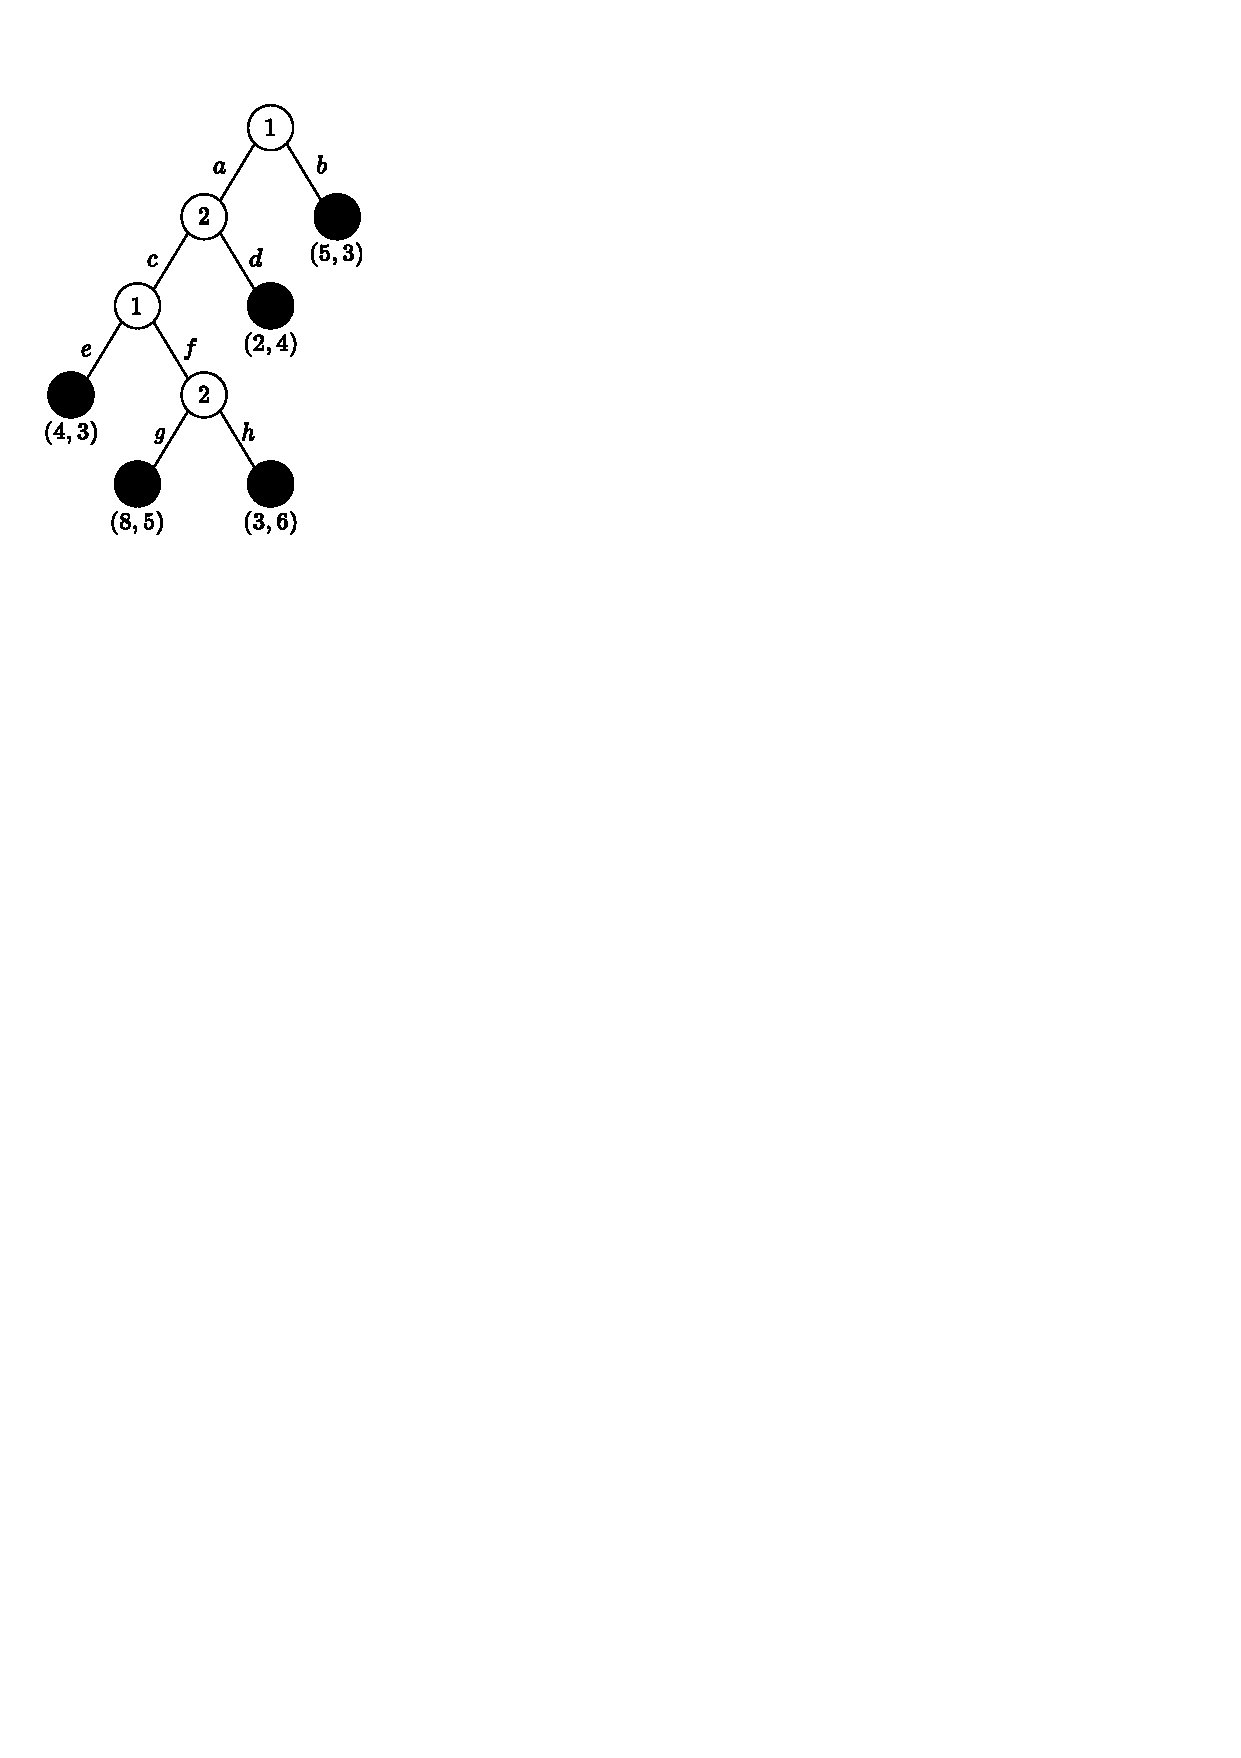
\includegraphics[scale=1]{经济博弈论3.5_1.pdf}
        \end{minipage}
    }
    \subfigure[] {
        \label{fig-5.2}
        \begin{minipage}[b]{.45\linewidth}
            \centering
            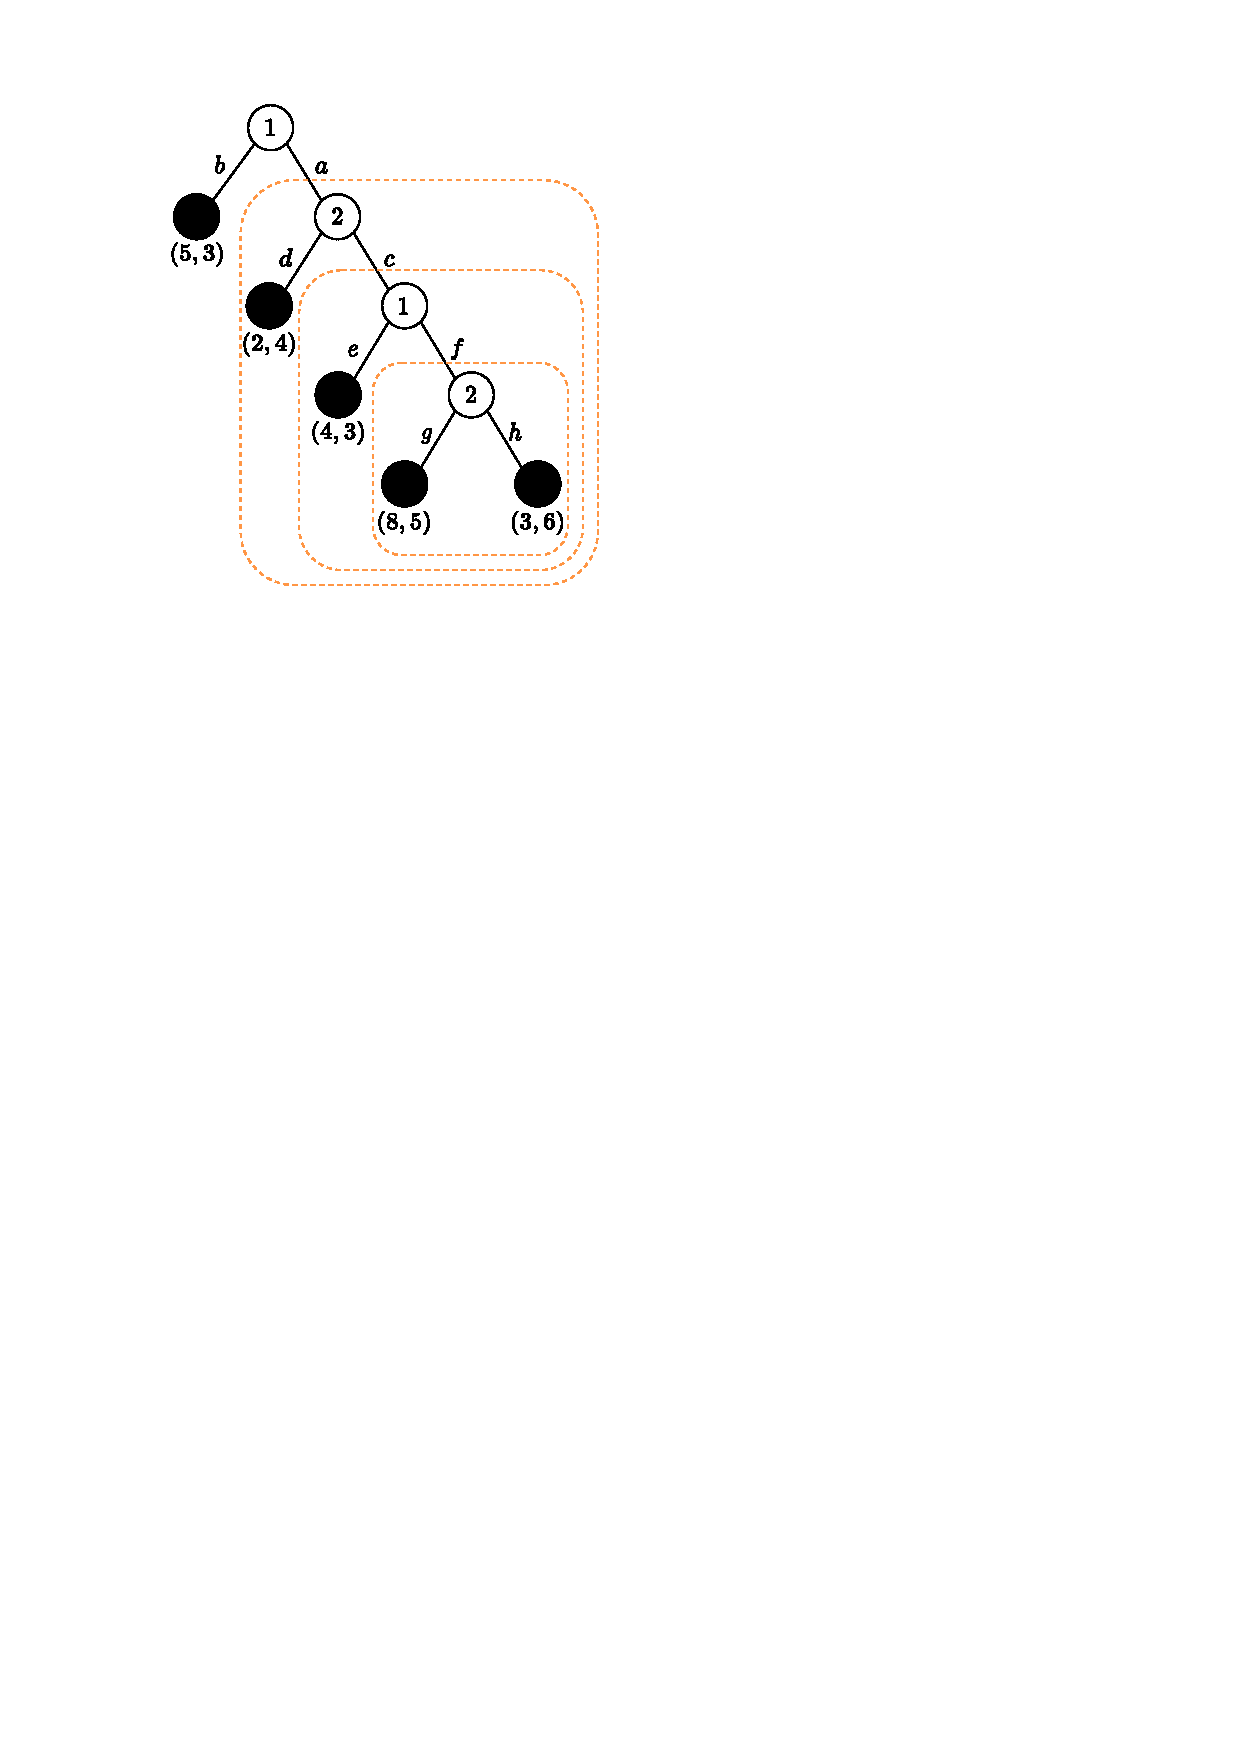
\includegraphics[scale=1]{经济博弈论3.5_2.pdf}
        \end{minipage}
    }
\end{figure}\del
\begin{solution}
    该博弈包含$3$个子博弈, 分别如图\ref{sub@fig-5.2}所示, 分别为: 第一阶段博弈方1选$a$开始的三阶段动态博弈; 第二阶段博弈方2选$c$开始的二阶段动态博弈; 第三阶段博弈方1选$f$开启的单人博弈.

    该博弈中最理想的解为$(8,5)$, 即决策路线为$a,c,f,g$. 但在第四阶段对于博弈方2会选择利益更大的$h$策略; 将得益$(3,6)$逆推到第三阶段, 对于博弈方1会选择利益更大的$e$策略; 将得益$(4,3)$逆推到第二阶段, 对于博弈方2会选择利益更大的$d$策略; 将得益$(2,4)$逆推到第一阶段, 对于博弈方1会选择利益更大的$b$策略. 综上决策路径$a,c,f,g$的每一步都不可信.

    根据上文说明可信性问题中使用逆推归纳法可知, 该博弈的完美纳什均衡策略组合为: 博弈方1于阶段一、三分别选$b, e$, 博弈方2于阶段二、四分别选$d, h$.
    
    博弈结果为博弈方1第一阶段选$b$, 博弈结束, 双方得益为$(5,3)$.
\end{solution}

\paragraph{6.}三寡头市场有倒转的需求函数$P = 100-Q$, 其中$Q$是$3$个厂商的产量之和, 并且已知$3$个厂商都有常数边际成本$2$而无固定成本. 如果厂商1和2同时决定产量, 厂商3根据厂商1和2的产量决策, 求它们的子博弈完美纳什均衡产量和相应的利润.
\begin{solution}
    设厂商1,2,3的产量分别为$h_1,\ h_2,\ h_3$, 则它们的利润函数分别为
    \begin{equation}\label{eq-w}
        w_i = (P-2)h_i = (98 - h_1-h_2-h_3)h_i,\quad(i = 1, 2, 3)
    \end{equation}
    用逆推归纳法分析该博弈, 在第二阶段, 假设厂商1,2已确定产量$h_1,h_2$, 则问题转化为厂商3单人博弈问题, 即以下最大化问题并求解, 可得厂商3的产量$h_3^*$
    \begin{equation}\label{eq-3}
        \max_{h_3\geq 0}w_3 = (98 - h_1-h_2-h_3)h_3\ \Rightarrow\ h_3^* = \frac{1}{2}(98 - h_1 - h_2),
    \end{equation}
    在第一阶段, 厂商1,2需根据上式(\ref{eq-3})决定均衡产量$h_3^*$, 即求解以下两个最大化问题
    \begin{equation}
        \max_{h_i\geq 0}w_i = (98 - h_i-h_j^* - h_3^*)h_i,\quad(i, j = 1, 2,\  i\neq j)
    \end{equation}
    将公式(\ref{eq-3})代入到$w_i$中得
    \begin{equation*}
        w_i = (98 - h_i - h_j^* -\frac{1}{2}(98-h_i-h_j^*))h_i = \frac{1}{2}(98-h_i-h_j^*)h_i,
    \end{equation*}
    最大化$w_i$可得
    \begin{equation*}
        \begin{cases}
            h_1^* = \frac{1}{2}(98 - h_2^*),\add\\
            h_2^* = \frac{1}{2}(98 - h_1^*).
        \end{cases}\Rightarrow\quad h_1^* = h_2^* = \frac{98}{3},
    \end{equation*}
    再代入到公式(\ref{eq-3})中, 可得$h_3^* = \frac{49}{3}$.\add
    
    综上, 它们的子博弈完美纳什均衡和相应的利润为
    \begin{equation*}
            h_1^* = h_2^* = \frac{98}{3},\quad h_3^* = \frac{49}{3},\quad
            w_1=w_2=\frac{4802}{9},\quad w_3 = \frac{2401}{3}.
    \end{equation*}
\end{solution}\del\del
\paragraph{7.}求下列得益矩阵表示的对称博弈的颤抖手均衡.
\begin{figure}[htbp]
    \centering
    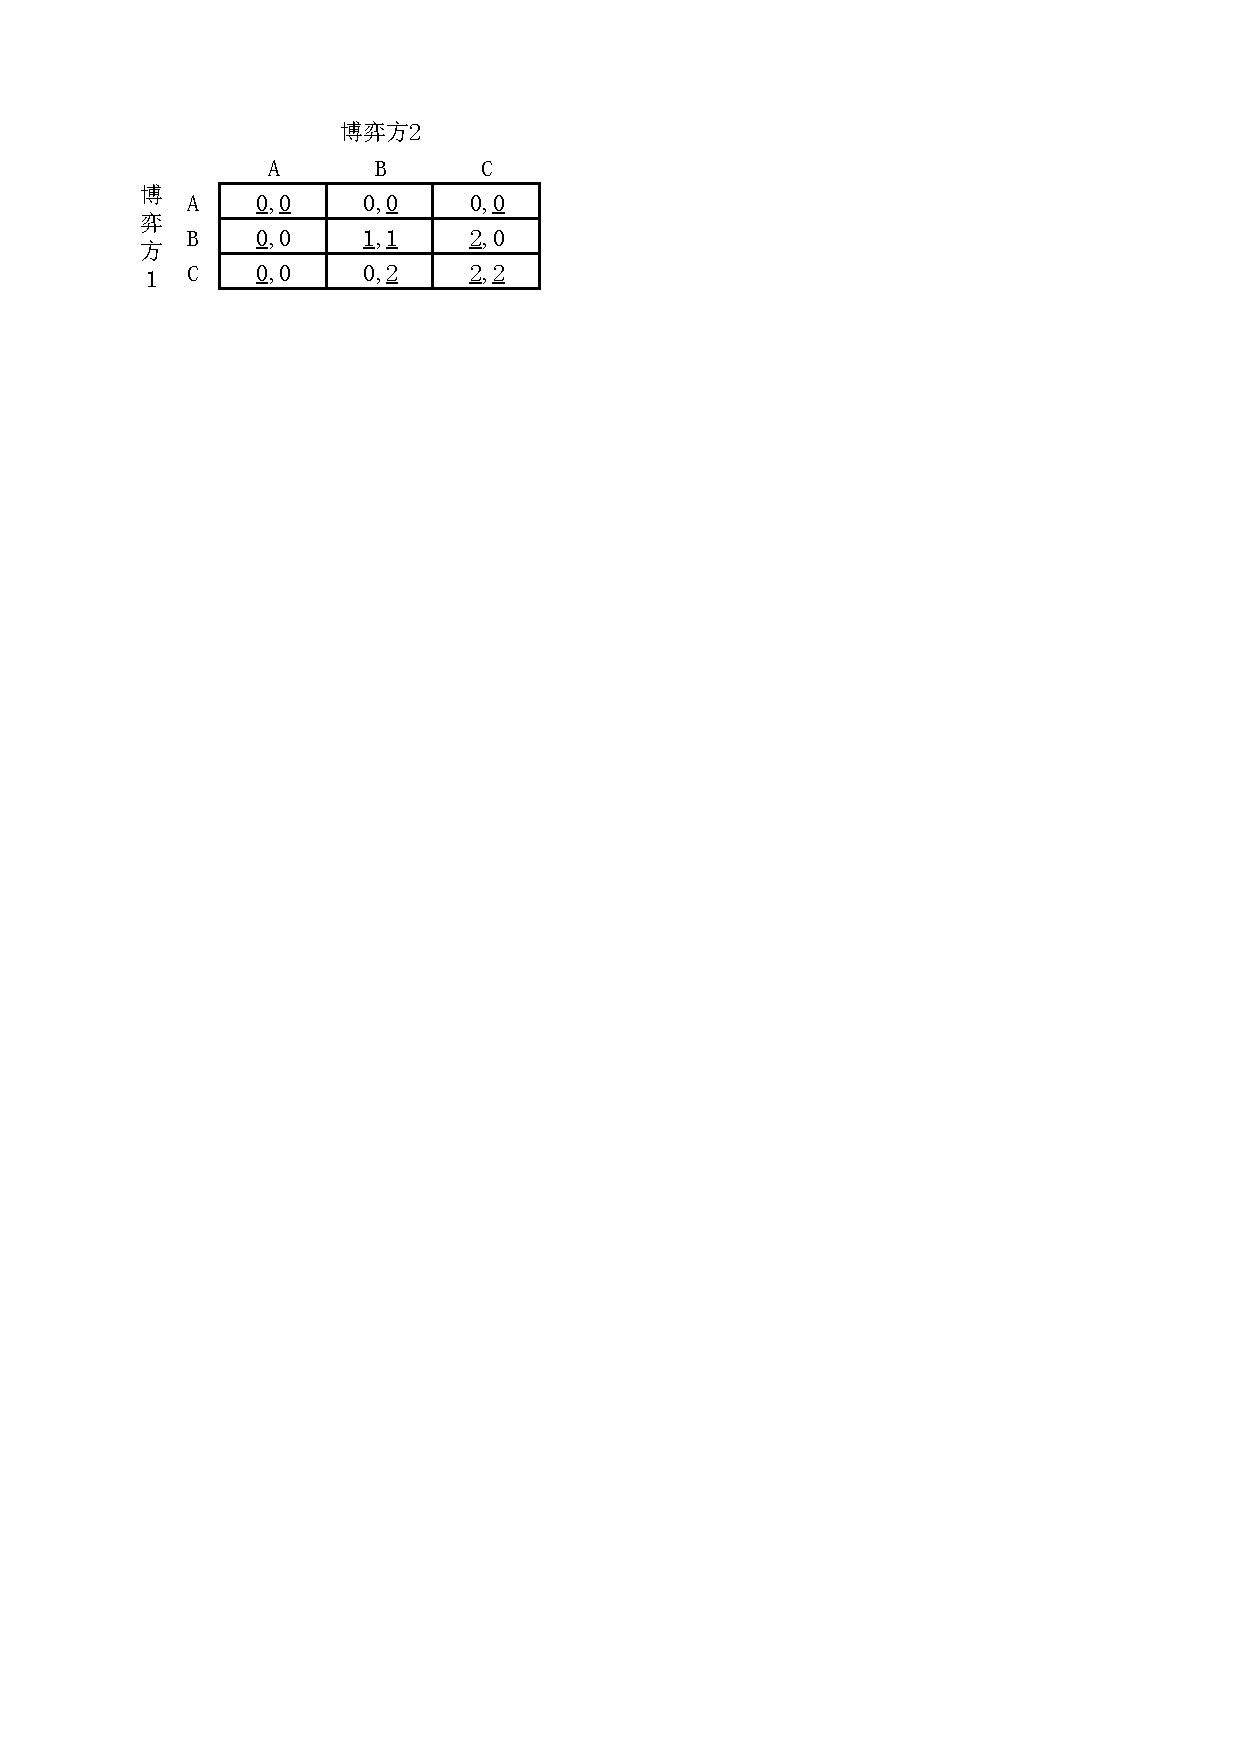
\includegraphics[scale=1]{经济博弈论3.7.pdf}
\end{figure}
\begin{solution}
    根据划线法可以确定策略$(A,A)$, $(B,B)$和$(C,C)$三个纯策略纳什均衡, 且$(C, C)$为Pareto均衡, 若都是完全理性博弈方, 则会选择决策$(C, C)$, 双方得益为$(2, 2)$.

    但考虑到博弈方可能犯错, 如果博弈方1认为博弈方2可能会犯错选择方案$A, B$, 如果博弈方2选择方案$B$, 则博弈方1以选择方案$B$的得益会大于选择方案$C$带来的损失, 则会选择方案$B$; 而且博弈方1也认为博弈方2考虑到对方也会犯错误, 从而也选择方案$B$, 且在方案$(B,B)$中, 任何一方故意犯错都不会增加自身的得益, 所以方案$(B,B)$为该得益矩阵的颤抖手均衡.
\end{solution}

% 下面给一些功能的写法
\iffalse
% 图片模板
\centerline{
    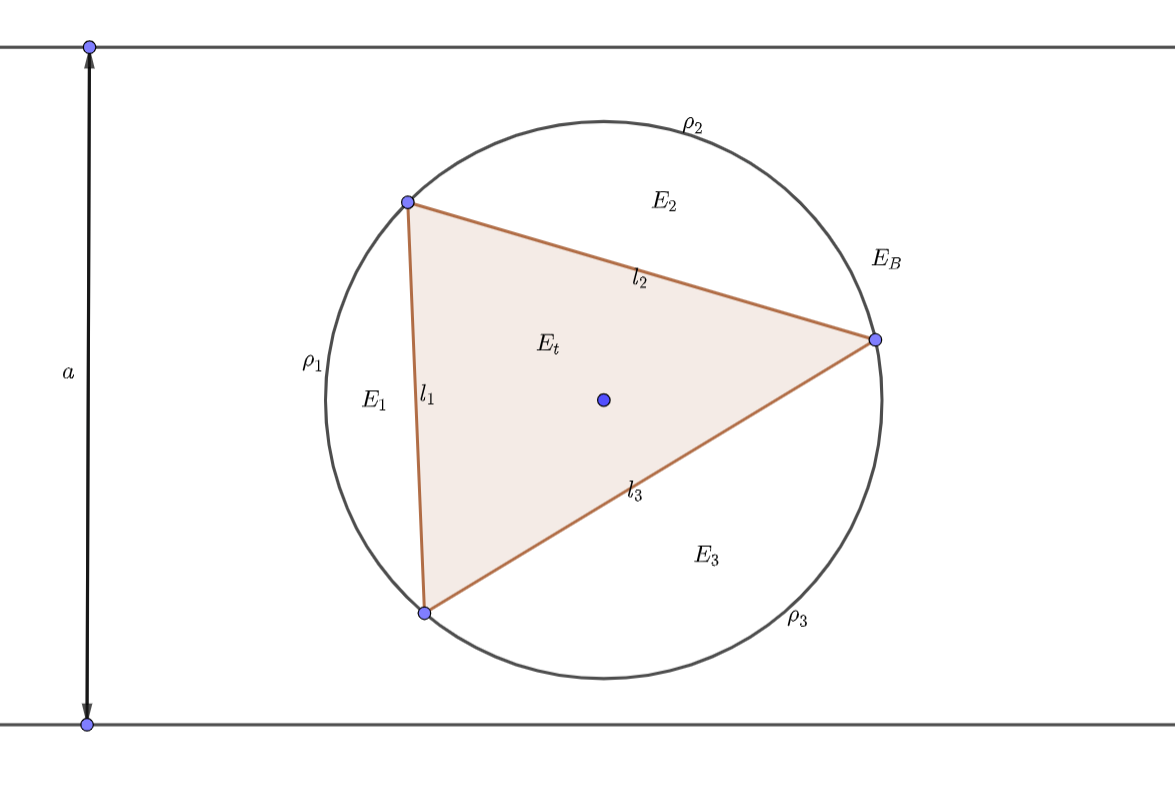
\includegraphics[width=0.8\textwidth]{figure.png}
}
% 表格模板
\renewcommand\arraystretch{0.8} % 设置表格高度为原来的0.8倍
\begin{table}[!htbp] % table标准
    \centering % 表格居中
    \begin{tabular}{p{1cm}<{\centering}p{1cm}<{\centering}p{3cm}<{\centering}p{5cm}<{\centering}} % 设置表格宽度
    %\begin{tabular}{cccc}
        \toprule
        $x_i$ & $f[x_1]$ & $f[x_i,x_{i+1}]$ & $f[x_i,x_{i+1},x_{i+2}]$ \\
        \midrule
        $x_0$ & $f(x_0)$ &                  &                          \\
        $x_0$ & $f(x_0)$ & $f'(x_0)$        &                          \\
        $x_0$ & $f(x_1)$ & $\frac{f(x_1)-f(x_0)}{x_1-x_0}$ & $\frac{f(x_1)-f(x_0)}{(x_1-x_0)^2}-\frac{f'(x_0)}{x_1-x_0}$\\
        \bottomrule
    \end{tabular}
\end{table}

\def\Log{\text{Log}} % 一个简单的宏定义
$\Log$ % 调用方法
\fi

\end{document}